
\begin{exercise} Consider a pair of circles $\mathcal{C}_R$ and $\mathcal{C}_r$ of radius $R>r$ and centered at $F_1$ and $F_2$ such that $|F_1-F_2|+r<R$. Consider the locus of center of bitangent circles. Show that this locus is an ellipse and find the semi-axes.
   
\end{exercise}

\begin{exercise}

\label{exerc:08-02-periodicsequence}
Consider the pair of confocal conics ($\E_1$, $\E_2$, $\Hc_1$ and $\Hc_2$) as shown in  \cref{fig:retangulo_exerc82}.

  Consider a ray starting at $F_1$ intersecting the branch $\Hc_2$ at $P_1$ and  the ray
  $F_2P_1$  intersecting the ellipse $\E_2$  at $P_2$. Analogously, we define the points $P_3=P_2F_1\cap\Hc_1$, $P_4=P_3F_2\cap\E_1$, $P_5=P_4F_1\cap\Hc_2$,
  $P_6$, etc.  
  
\noindent i) Determine conditions to obtain $P_5=P_1$. 
In this case show that the perimeter of the quadrilateral
$P_1P_2P_3P_4$ is constant, i.e., independent of the position of the point $P_1$.  See \cite{dolgirev2014}.


\noindent ii) Analyze the cases when $P_1=\E_2\cap \Hc_2$ or $P_1=\E_1\cap \Hc_2$.

 \begin{figure}[H]
 	\begin{center}
 	 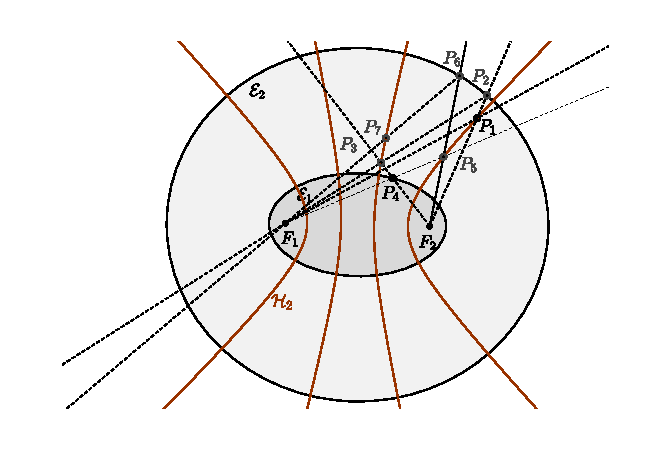
\includegraphics[scale=1]{chap_09/pics/pics_09_910_dinamica_retangulos.pdf}
 		\caption {Sequence of points $P_1,  \,P_2, \ldots,  P_5 ,  \ldots$  
 		 \label{fig:retangulo_exerc82} }
 	\end{center}
 	\end{figure}
 	
 	\end{exercise}
 	
 	
\begin{exercise} See \cite{izmestiev2017-ivory} and \cite{stachel-ivory-2019}.
   Given a confocal family of conics   in each Ivory quadrangle $PP'Q'Q$ inscribed in a pair of ellipses $\{\E_1,\E_2\}$
with diagonals $PQ'$ and $QP'$ tangent to  $\E_c$ all billiards (defined in the quadrangle $PP'Q'Q$) with sidelines
being tangent to $\E_c$ are closing and have equal lengths. See \cref{fig:09-ivory-4billiard}.
\begin{figure}
    \centering
    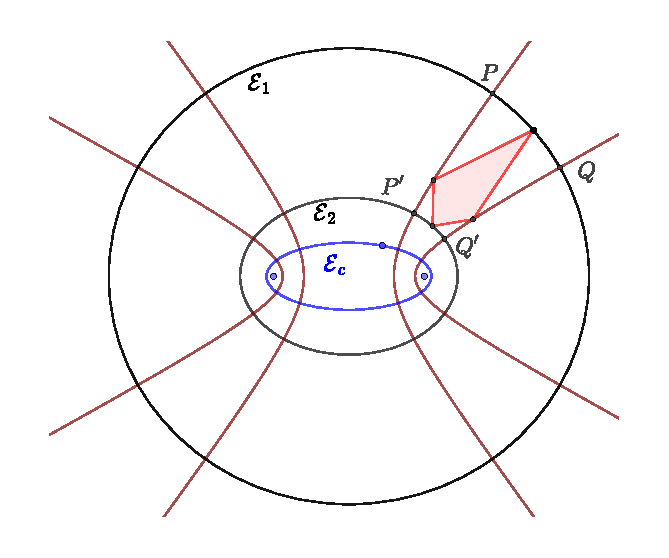
\includegraphics[scale=0.5]{pics-09-130-ivory-4billiard.pdf}
    \caption{A 4-periodic billiard orbit (red) in the quadrangle $PP'QQ'$ with diagonals tangent to $\mathcal{E}_c$.}
    \label{fig:09-ivory-4billiard}
\end{figure}
\end{exercise}

\begin{exercise}
Consider a triangle $T=ABC$ inscribed in an ellipse with semi-axes $a$ and $b$. Consider the three diameters $A'A''$, $B'B''$ and $C' C''$ as shown in \cref{fig:pics-09-200-3cordas}. Show that the radius of the circumcircle of $T$ is given by
\[R=\frac{ |A'-A''| |B'-B''| |C'-C''| }{8ab}\]

\end{exercise}

\begin{figure}
    \centering
    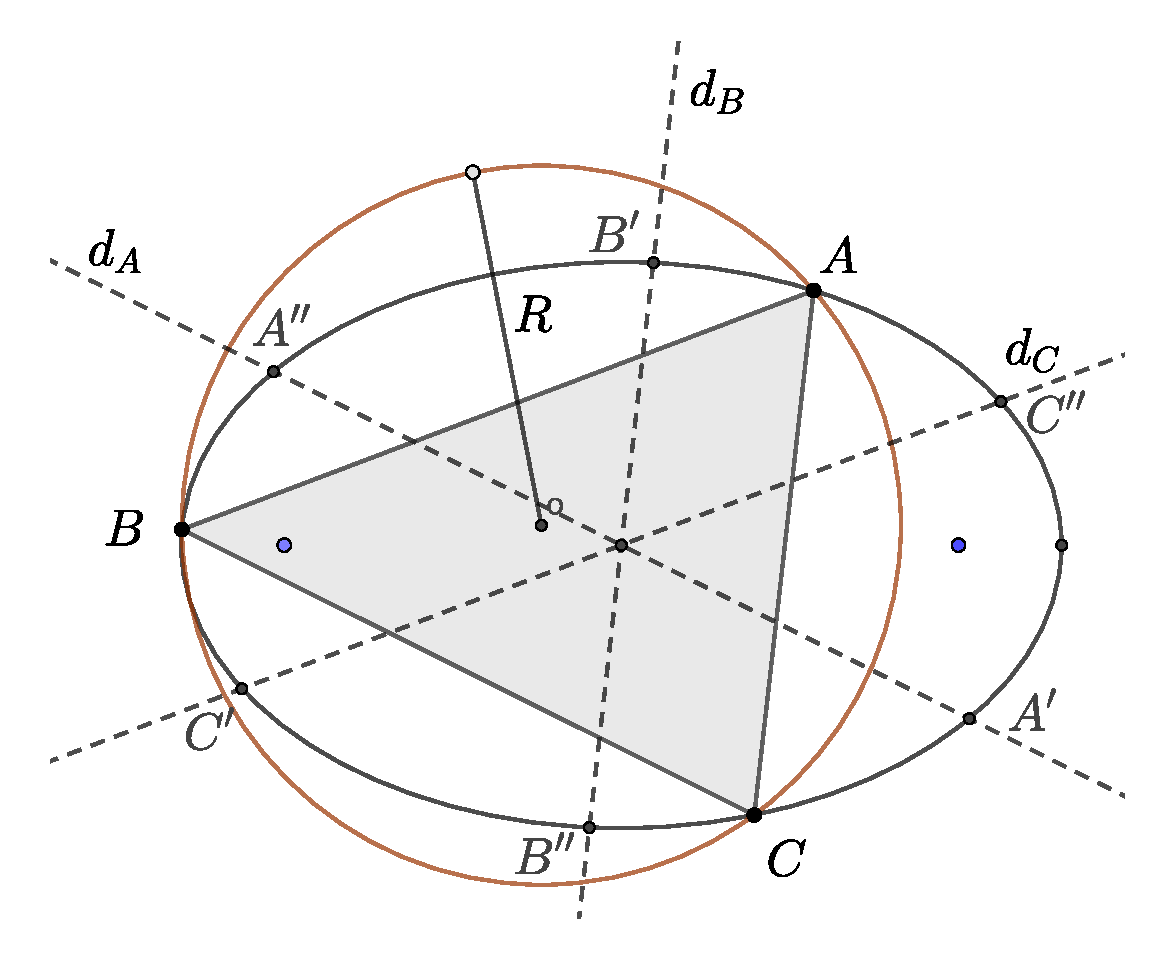
\includegraphics[scale=0.5]{ii_chap_09/pics/pics-09-200-triangleA_3diametros.pdf}
    \caption{ Diameters of chords and circumcircle of a triangle inscribed in an  ellipse.}
    \label{pics-09-200-3cordas}
\end{figure}

\begin{exercise}
Show that  for any point $P_0$ in an ellipse, there exists three distinct points  $P_1,\, P_2,\, P_3$  in   the same ellipse such $P_0$ is a point in the intersection of three osculating circles passing through  $P_1,\, P_2,\, P_3$. Show that the four points $P_i$ are concircular.
See \cref{fig:09-3osculador}.

\end{exercise}

\begin{figure}
    \centering
    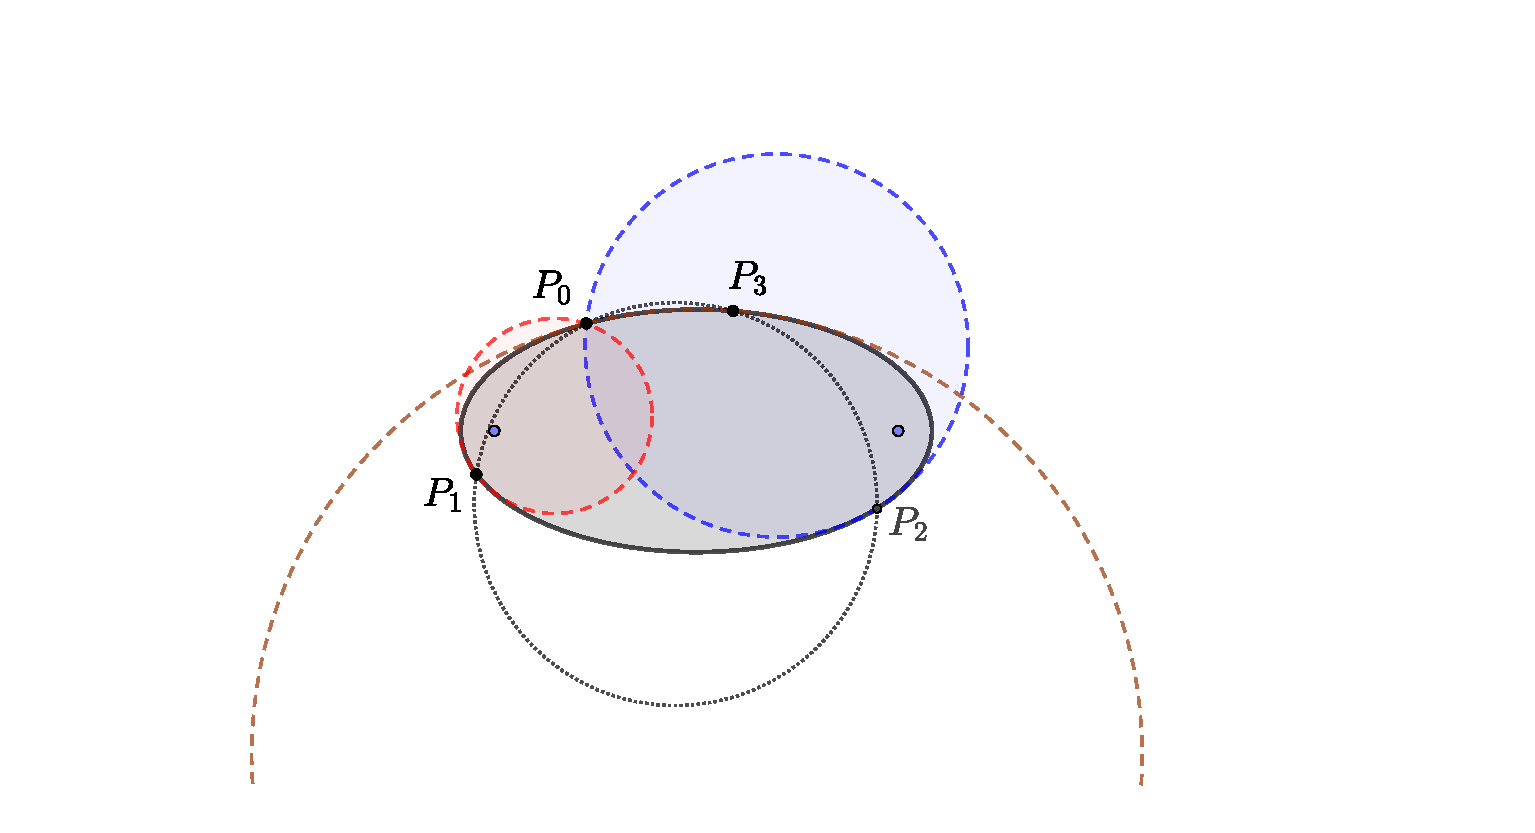
\includegraphics[width=0.7]{ii_chap_09/pics/pics_09_210_3osculador.pdf}
    \caption{Three osculating circles passing through a given point $P_0$.}
    \label{fig:09-3osculador}
\end{figure}
    
 